\documentclass{memoir}
\usepackage{notestemplate}
\usetikzlibrary{arrows,chains,matrix,positioning,scopes}

\makeatletter
\tikzset{join/.code=\tikzset{after node path={%
\ifx\tikzchainprevious\pgfutil@empty\else(\tikzchainprevious)%
edge[every join]#1(\tikzchaincurrent)\fi}}}
\makeatother

\tikzset{>=stealth',every on chain/.append style={join},
         every join/.style={->}}

%\logo{~/School-Work/Auxiliary-Files/resources/png/logo.png}
%\institute{Rice University}
%\faculty{Faculty of Whatever Sciences}
%\department{Department of Mathematics}
%\title{Class Notes}
%\subtitle{Based on MATH xxx}
%\author{\textit{Author}\\Gabriel \textsc{Gress}}
%\supervisor{Linus \textsc{Torvalds}}
%\context{Well, I was bored...}
%\date{\today}

%\makeindex

\begin{document}

% \maketitle

% Notes taken on 06/08/21

Consider modules \(A,C\). One question worth exploring is if there exists a module \(B\) such that \(A / B \cong C\); that is, \(B\) is an extension of \(C\) by \(A\). The tools we develop to understand this question are exact sequences. If \(A\) is isomorphic to a submodule of \(B \), there is an injective homomorphism from \(A\) to \(B\). And if \(C\) is isomorphic to the quotient, then there is a surjective homomorphism from \(B\) to \(C\). This will give us a chain
\begin{align*}
	A \to B \to C
\end{align*}
where the homomorphisms are compatible with. We formalize this idea via exact sequences.

\begin{defn}[Exact Sequences]
	Let \(\alpha ,\beta \) be homomorphisms so that
	\begin{align*}
		X \to^{\alpha } Y \to^{\beta }Z.
	\end{align*}
	If \(\textrm{Im}(\alpha ) = \textrm{Ker}(\beta )\), then we say the pair of homomorphisms are \textbf{exact}.\\

	A sequence of homomorphisms
	\begin{align*}
		\ldots \to X_{n-1} \to X_n \to X_{n+1} \to \ldots
	\end{align*}
	is said to be an \textbf{exact sequence} if it is exact at every \(X_n\) between a pair of homomorphisms.
\end{defn}
Hence, our goal is to see whether we can form an exact sequence \(A\to B\to C\). Our notions of injectivity and surjectivity correspond exactly to the notions of exactness.
\begin{prop}
	Let \(A,B,C\) form \(R\)-modules over some ring \(R\). Then the sequence
	\begin{align*}
		0 \to A \to^{\psi }B
	\end{align*}
	is exact at \(A\) if and only if \(\psi \) is injective. Likewise, the sequence
	\begin{align*}
		B \to^{\varphi }\to C \to 0
	\end{align*}
	is exact at \(C\) if and only if \(\varphi \) is surjective.
\end{prop}
Combining the two ideas, the sequence
\begin{align*}
	0 \to A \to^{\psi }B \to^{\varphi }C \to 0
\end{align*}
is exact if and only if \(\psi \) is injective, \(\varphi \) is surjective, and \(\textrm{Im}(\psi ) = \textrm{Ker}(\varphi )\).

\begin{defn}
	An exact sequence of the form
	\begin{align*}
		0 \to A \to^{\psi }B \to^{\varphi }C \to 0
	\end{align*}
	is called an \textbf{short exact sequence}.
\end{defn}
Our goal then is to determine if two modules admit a short exact sequence, and if so, how many.\\

Notice that any exact sequence can be written as a succession of short exact sequences. For example, if
\begin{align*}
	X \to^{\alpha }Y \to^{\beta }Z
\end{align*}
is exact at \(Y\), then equivalently
\begin{align*}
	0 \to \alpha (X) \to Y \to Y / \textrm{Ker}(\beta ) \to 0
\end{align*}
is a short exact sequence.

\begin{exmp}
	
\end{exmp}

For fixed \(A,C\), there can be many extensions of \(C\) by  \(A\). Hence, we need to determine a notion of a homomorphism to distinguish exact sequences.

\begin{defn}[Homomorphism of Short Exact Sequences]
	Let
	\begin{align*}
		0 \to A \to B \to C \to 0\\
		0 \to A' \to B' \to C' \to 0
	\end{align*}
	be two short exact sequences of modules. A \textbf{homomorphism of short exact sequences} is a collection of module homomorphisms \(\alpha ,\beta ,\gamma \) such that the following diagram commutes:
\begin{center}
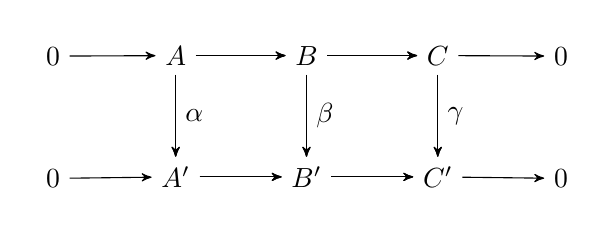
\begin{tikzpicture}
  \matrix (m) [matrix of math nodes, row sep=3em, column sep=3em]
    { 0 & A  & B  & C  & 0 \\
      0 & A' & B' & C' & 0 \\ };
  { [start chain] \chainin (m-1-1);
    \chainin (m-1-2);
    { [start branch=A] \chainin (m-2-2)
        [join={node[right] {$\alpha $}}];}
    \chainin (m-1-3) [join={node[above] {}}];
    { [start branch=B] \chainin (m-2-3)
        [join={node[right] {$\beta $}}];}
    \chainin (m-1-4) [join={node[above] {}}];
    { [start branch=C] \chainin (m-2-4)
        [join={node[right] {$\gamma $}}];}
    \chainin (m-1-5); }
  { [start chain] \chainin (m-2-1);
    \chainin (m-2-2);
    \chainin (m-2-3) [join={node[above] {}}];
    \chainin (m-2-4) [join={node[above] {}}];
    \chainin (m-2-5); }
\end{tikzpicture}
\end{center}
This is an \textbf{isomorphism of short exact sequences} if \(\alpha ,\beta ,\gamma \) are isomorphisms in which case the extensions \(B,B'\) are \textbf{isomorphic extensions}.\\

The two exact sequences are called \textbf{equivalent} if \(A = A'\), \(C = C'\), and there is an isomorphism between them where  \(\alpha ,\gamma \) are identity. In this case \(B\) and \(B'\) are \textbf{equivalent extensions}.
\end{defn}
Equivalency by extensions is stronger than just \(R\)-module isomorphisms between \(B\) and \(B'\)-- it tells us tat there is an \(R\)-module isomorphism between \(B\) and \(B'\) that restricts to an isomorphism from \(A\) to \(A'\) and induces an isomorphism on the quotients by \(C\) and \(C'\).

\begin{exmp}
	
\end{exmp}

\begin{prop}[Short Five Lemma]
	Let \(\alpha ,\beta ,\gamma \) be a homomorphism of short exact sequences
\begin{center}
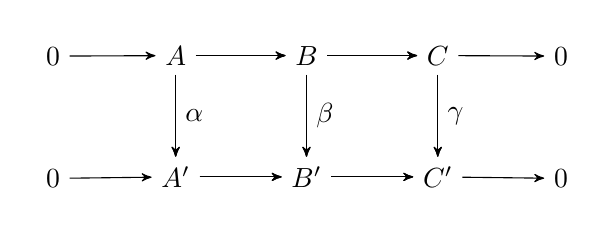
\begin{tikzpicture}
  \matrix (m) [matrix of math nodes, row sep=3em, column sep=3em]
    { 0 & A  & B  & C  & 0 \\
      0 & A' & B' & C' & 0 \\ };
  { [start chain] \chainin (m-1-1);
    \chainin (m-1-2);
    { [start branch=A] \chainin (m-2-2)
        [join={node[right] {$\alpha $}}];}
    \chainin (m-1-3) [join={node[above] {}}];
    { [start branch=B] \chainin (m-2-3)
        [join={node[right] {$\beta $}}];}
    \chainin (m-1-4) [join={node[above] {}}];
    { [start branch=C] \chainin (m-2-4)
        [join={node[right] {$\gamma $}}];}
    \chainin (m-1-5); }
  { [start chain] \chainin (m-2-1);
    \chainin (m-2-2);
    \chainin (m-2-3) [join={node[above] {}}];
    \chainin (m-2-4) [join={node[above] {}}];
    \chainin (m-2-5); }
\end{tikzpicture}
\end{center}
\begin{itemize}
	\item If \(\alpha ,\gamma \) are injective then so is \(\beta \) 
	\item If \(\alpha ,\gamma \) are surjective then so is \(\beta \) 
	\item If \(\alpha ,\gamma \) are isomorphisms then so is \(\beta \)
\end{itemize}
\end{prop}
These results also hold for short exact sequences of groups.

\begin{proof}[Proof of Short Five Lemma]
	
\end{proof}
There is always at least one extension of a module \(C\) by \(A\) given by \(B = A \oplus C\).

\begin{defn}
	Let \(R\) be a ring and let
	\begin{align*}
		0 \to A \to^{\psi }B \to^{\varphi }C \to 0
	\end{align*}
	be a short exact sequence of \(R\)-modules. We say the sequence is \textbf{split} if there is an \(R\)-module complement to \(\psi (A)\) in \(B\). If this holds, then \(B = A \oplus C\) up to isomorphism by
	\begin{align*}
		B = \psi (A) \oplus C'
	\end{align*}
	for some submodile \(C'\), where \(\varphi (C') \cong C\).\\

	We say \(B\) is a \textbf{split extension of \(C\) by \(A\)}.
\end{defn}
This is really just the question of existence of a complement to \(\psi (A)\) in \(B\) that is isomorphic by \(\varphi \) to \(C\).

\begin{prop}
	The short exact sequence
	\begin{align*}
		0 \to A \to^{\psi }B \to^{\varphi }C \to 0
	\end{align*}
	of \(R\)-modules is split if and only if there is an \(R\)-module homomorphism \(\mu :C \to B\) such that \(\varphi \circ \mu \cong \textrm{Id}_C\).\\

	Any set map \(\mu :C\to B\) such that \(\varphi \circ \mu = \textrm{Id}_C\) is called a \textbf{section} of \(\varphi \). If \(\mu \) is a homomorphism, then \(\mu \) is called a \textbf{splitting homomorphism} for the sequence.
\end{prop}
A section of \(\varphi \) is merely a choice of coset representative in \(B\) for \(B / \textrm{Ker}\varphi  \cong C\). A section is a homomorphism if this set of coset representatives forms a submodule, in which case this submodule gives a complement to \(\psi (A)\) in \(B\).

\begin{exmp}
	
\end{exmp}

\begin{prop}
	Let
	\begin{align*}
		0 \to A \to^{\psi }B \to^{\varphi }C \to 0
	\end{align*}
	be a short exact sequence of modules. Then \(B = \psi (A) \oplus C'\) for some submodule \(C'\) of \(B\) with \(\varphi (C') \cong C\) if and only if there is a homomorphism \(\lambda :B\to A\) such that \(\lambda \circ \psi = \textrm{Id}_A\) .
\end{prop}
For groups, this is a stronger notion. The existence of a splitting homomorphism on the left end of the sequence gives that the extension group is a direct product (instead of a semidirect product). Of course, in modules there is no distinction as the underlying groups are abelian.

\subsection{Projective Modules}
\label{sub:projective_modules}

Let \(R\) be a ring and suppose that \(\prescript{}{R}M\) is an extension of \(N\) by \(L\), so that
\begin{align*}
	0 \to L \to^{\psi }M \to^{\varphi }N \to 0.
\end{align*}
If another \(R\)-module has an \(R\)-module homomorphism into \(L\) or \(N\), can it extend to a homomorphism to \(M\)?\\

We can see directly that if \(f \in \textrm{Hom}_R(D,L)\) then \(f' = \psi \circ f\) is an \(R\)-module homomorphism from \(D\) to \(M\):
\begin{align*}
	\psi': \textrm{Hom}_R(D,L) \to \textrm{Hom}_R(D,M)\\
	f \mapsto f' = \psi \circ f.
\end{align*}

\begin{prop}
	Let \(D,L,\) and \(M\) form \(R\)-modules and let \(\psi :L \to M\) be an \(R\)-module homomorphism. Then the map
	\begin{align*}
		\psi': \textrm{Hom}_R(D,L) &\to \textrm{Hom}_R(D,M)\\
		f &\mapsto f' = \psi \circ f
	\end{align*}
	is a homomorphism of abelian groups. If \(\psi \) is injective, then \(\psi '\) is injective. Hence, if
	\begin{align*}
		0 \to L \to^{\psi }M
	\end{align*} is exact, then
	\begin{align*}
		0 \to \textrm{Hom}_R(D,L) \to^{\psi '} \textrm{Hom}_R(D,M)
	\end{align*}
	is exact.
\end{prop}

Unfortunately, if there is an \(R\)-module homomorphism \(f:D \to N\), it isn't always the case that \(f\) \textbf{lifts} to an \(R\)-module homomorphism \(f:D\to M\) by
\begin{align*}
	\varphi ': \textrm{Hom}_R(D,M) &\to \textrm{Hom}_R(D,N)\\
	F &\mapsto F' = \varphi \circ F
\end{align*}
This only holds if and only if \(f\) is in the image of \(\varphi '\).

\begin{exmp}
	
\end{exmp}

\begin{thm}
	Let \(D,L,M,N\) form \(R\)-modules. If
	\begin{align*}
		0 \to L \to^{\psi }M \to^{\varphi }N \to 0
	\end{align*}
	is exact, then
	\begin{align*}
		0 \to \textrm{Hom}_R(D,L) \to^{\psi '} \textrm{Hom}_R(D,M) \to^{\varphi '} \textrm{Hom}_R(D,N)
	\end{align*}
	is exact.\\

	A homomorphism \(f:D\to N\) lifts to a homomorphism \(F:D\to M\) if and only if \(f \in \textrm{Hom}_R(D,N)\) is in the image of \(\varphi '\). In general \(\varphi '\) is surjective if and only if every homomorphism from \(D\) to \(N\) lifts to a homomorphism from \(D\) to \(M\), in which case the sequence above extends to a short exact sequence.\\

	The sequence above is exact for all \(R\)-modules \(D\) if and only if
	\begin{align*}
		0 \to L \to^{\psi }M \to^{\varphi }N
	\end{align*}
	is exact.
\end{thm}
Hence, by the theorem, the sequence
\begin{align*}
	0 \to \textrm{Hom}_R(D,L) \to^{\psi '}\textrm{Hom}_R(D,M) \to^{\varphi '} \textrm{Hom}_R(D,N) \to 0
\end{align*}
is in general not a short exact sequence, as \(\varphi '\) may not be surjective. In fact, this sequence is exact if and only if there is a bijection between homomorphisms \(F:D \to M\) and \(g:D\to L\), \(f:D\to N\) where
\begin{align*}
	F\mid_{\varphi (L)} = \psi'(g)\\
	f = \varphi'(F).
\end{align*}
Notice that if the original sequence is spit exact, then the sequence of homomorphisms is also split exact.
\begin{prop}
	Let \(D,L,N\) form \(R\)-modules. Then
	\begin{align*}
		\textrm{Hom}_R(D,L\oplus N) \cong \textrm{Hom}_R(D,L) \oplus \textrm{Hom}_R(D,N)\\
		\textrm{Hom}_R(L \oplus N, D) \cong \textrm{Hom}_R(L,D) \oplus \textrm{Hom}_R(N,D)
	\end{align*}
\end{prop}
Of course this extends by induction to any finite direct sum of \(R\)-modules. In other words, the group of module homomorphisms commute with dfinite direct sums in either variable.

\begin{rmrk}
	For infinite direct sums, this does not always hold. If \(L \oplus N\) is replaced by an arbitrary direct sum, and the direct sum on the right hand side is replaced by a direct product, then
	\begin{align*}
		\textrm{Hom}_R(D,L\oplus \left\{ N_i \right\}_{i \in I}) \cong \textrm{Hom}_R(D,L) \otimes \left\{ \textrm{Hom}_R(D,N_i) \right\}_{i \in I} 
	\end{align*}
	holds. The second part must be translated into
	\begin{align*}
		\textrm{Hom}_R(L \otimes \left\{ N_i \right\}_{i \in I},D) \cong \textrm{Hom}_R(L,D) \otimes \left\{ \textrm{Hom}_R(N_i,D) \right\}_{i \in I}
	\end{align*}
\end{rmrk}

Hence, a split short exact sequence of \(R\)-modules induces a split short exact sequence of abelian groups for every \(R\)-module \(D\). In fact, the converse holds:
\begin{hw}
	Prove that if
	\begin{align*}
		0 \to \textrm{Hom}_R(D,L) \to^{\psi '} \textrm{Hom}_R(D,M) \to^{\varphi'} \textrm{Hom}_R(D,N) \to 0
	\end{align*} is exact for every \(R\)-module \(D\), then
	\begin{align*}
		0 \to L \to^{\psi }M \to^{\varphi }N \to 0
	\end{align*}
	is a split short exact sequence.\\

	This implies that if the original homomorphism sequence is exact for every \(D\), then it is in fact split exact for every \(D\).
\end{hw}

\begin{prop}
	Let \(P\) be an \(R\)-module. Then the following are equivalent:
	\begin{itemize}
		\item Let \(L,M,N\) form \(R\)-modules. If
			\begin{align*}
				0 \to L \to^{\psi }M \to^{\varphi }N \to 0
			\end{align*}
			is a short exact sequence, then
			\begin{align*}
				0 \to \textrm{Hom}_R(P,L) \to^{\psi '} \textrm{Hom}_R(P,M) \to^{\varphi '} \textrm{Hom}_R(P,N) \to 0
			\end{align*}
			is a short exact sequence.
		\item Let \(M,N\) form \(R\)-modules. If
			 \begin{align*}
				M \to^{\varphi }N \to 0
			\end{align*}
			is exact, then every \(R\)-module homomorphism from \(P\) into \(N\) lifts to an \(R\)-module homomorphism into \(M\), so the following diagram commutes:
\begin{center}
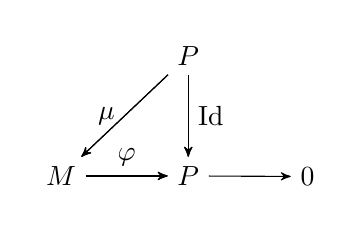
\begin{tikzpicture}% Fix later by making mu dashed
  \matrix (m) [matrix of math nodes, row sep=3em, column sep=3em]
    {  & P  &   \\
      M & P & 0 \\ };
  { [start chain];
    \chainin (m-1-2);
    { [start branch=P] \chainin (m-2-1)
        [join={node[left] {$\mu  $}}];}
    { [start branch=P'] \chainin (m-2-2)
	[join={node[right] {$\textrm{Id} $}}];}}
  { [start chain] \chainin (m-2-1);
    \chainin (m-2-2) [join={node[above] {\(\varphi \)}}];
    \chainin (m-2-3) ;}
\end{tikzpicture}
\end{center}
	\item If \(P\) is a quotient of the \(R\)-module \(M\) then \(P\) is isomorphic to a direct summand of \(P\). That is, every short exact sequence
		\begin{align*}
			0\to L \to M\to P\to 0
		\end{align*}
		splits.
	\item \(P\) is a direct summand of a free \(R\)-module.
	\end{itemize}
\end{prop}

\begin{defn}[Projective Modules]
	An \(R\)-module \(\prescript{}{R}P\) is called \textbf{projective} if any module \(M\) that projects onto \(P\) has an isomorphic copy of \(P\) as a direct summand.
\end{defn}
A projective module is merely one that satisfies any of the above equivalent conditions.

\begin{cor}
	Free modules are projective modules.\\

	A finitely generated module is projective if and only if it is the direct summand of a finitely generated free module.\\

	Every free module is a quotient of a projective module.
\end{cor}

\begin{exmp}
	
\end{exmp}

% Category theory explanation and functors

\subsection{Injective Modules}
\label{sub:injective_modules}

Of course we can also consider the reverse case-- when do \(R\)-module homomorphisms from \(L\) or \(N\) to \(D\) exist?\\

We can see that an \(R\)-module map from \(N\) to \(D\) induces a map from \(M\) to \(D\) by composition by
\begin{align*}
	\varphi' : \textrm{Hom}_R(N,D) &\to \textrm{Hom}_R(M,D)\\
	f &\mapsto f' = f \circ \varphi 
\end{align*}
which is injective, and hence if the sequence
\begin{align*}
	M\to^{\varphi }N \to 0
\end{align*} is exact, then
\begin{align*}
	0 \to \textrm{Hom}_R(N,D) \to^{\varphi '} \textrm{Hom}_R(M,D)
\end{align*} is exact.\\

The reverse does not hold in general.

\begin{exmp}
	
\end{exmp}

\begin{thm}
	Let \(D,L,M,N\) form \(R\)-modules. If
	\begin{align*}
		0 \to L \to^{\psi }M \to^{\varphi }N \to 0
	\end{align*}
	is exact, then
	\begin{align*}
		0 \to \textrm{Hom}_R(N,D) \to^{\varphi '} \textrm{Hom}_R(M,D) \to^{\psi'} \textrm{Hom}_R(L,D)
	\end{align*} is exact.\\

	A homomorphism \(f:L\to D\) lifts to a homomorphism \(F:M\to D\) if and only if \(f\) is in the image of \(\psi '\).\\

	The sequence of homomorphisms is exact for all \(R\)-modules \(D\) if and only if
	\begin{align*}
		L \to^{\psi }M \to^{\varphi }N \to 0
	\end{align*}
	is exact.
\end{thm}
Hence the sequence
\begin{align*}
	0 \to \textrm{Hom}_R(N,D) \to^{\varphi '}\textrm{Hom}_R(M,D) \to^{\psi '}\textrm{Hom}_R(L,D) \to 0
\end{align*} is not a short exact sequence in general, as \(\psi '\) may not be surjective.\\

Of course, this sequence is exact if the original exact sequence is a split exact sequence (in which case the sequence of homomorphisms is a split exact sequence for every \(R\)-module \(D\)).

\begin{hw}
	If 
	\begin{align*}
		0 \to \textrm{Hom}_R(N,D) \to^{\varphi '}\textrm{Hom}_R(M,D) \to^{\psi '}\textrm{Hom}_R(L,D) \to 0
	\end{align*}
	is exact for every \(R\)-module \(D\), then
	\begin{align*}
		0 \to L \to^{\psi }M \to^{\varphi }N \to 0
	\end{align*}
	is a split short exact sequence.\\

	This implies that if the homomorphism sequence is exact for every \(D\), then it is split exact for every \(D\).
\end{hw}

\begin{prop}
	Let \(Q\) be an \(R\)-module. Then the following are equivalent:
	\begin{itemize}
		\item Let \(L,M,N\) form \(R\)-modules. If
			\begin{align*}
				0 \to L \to^{\psi }M \to^{\varphi }N \to 0
			\end{align*}
			is a short exact sequence, then
			\begin{align*}
				0 \to \textrm{Hom}_R(N,Q) \to^{\varphi '} \textrm{Hom}_R(M,Q) \to^{\psi '} \textrm{Hom}_R(L,Q) \to 0
			\end{align*}
			is also a short exact sequence.
		\item Let \(L,M\) form \(R\)-modules. If \(0 \to L\to^{\psi }M\) is exact, then every \(R\)-module homomorphism from \(L\) to \(Q\) lifts to an \(R\)-module homomorphism of \(M\) into \(Q\). That is, the following diagram commutes:
\begin{center}
\begin{tikzpicture}% Fix later by making F dashed
  \matrix (m) [matrix of math nodes, row sep=3em, column sep=3em]
    { 0 & L  & M  \\
       & Q &  \\ };
  { [start chain];
    \chainin (m-1-1);
    \chainin (m-1-2);
    { [start branch=L] \chainin (m-2-2)
    [join={node[left] {\(f\) }}];}
    \chainin (m-1-3) [join={node[above] {\(\psi \)}}];
    { [start branch=M] \chainin (m-2-2)
	[join={node[right] {$F $}}];}}
\end{tikzpicture}
\end{center}
\item If \(Q\) is a submodule of the \(R\)-module \(M\), then \(Q\) is a direct summand of \(M\). That is, every short exact sequence
	\begin{align*}
		0 \to Q \to M \to N \to 0
	\end{align*}
	splits.
	\end{itemize}
\end{prop}

\begin{defn}[Injective Modules]
	An \(R\)-module \(\prescript{}{R}Q\) is called \textbf{injective} if for any module \(M\) that \(Q\) injects into, \(M\) has an isomorphic copy of \(Q\) as a direct summand.
\end{defn}

\begin{exmp}
		
\end{exmp}

%Category theory stuff again

Unfortunately, there is not a nice equivalent to the direct summand of a free \(R\)-module condition from projective modules. Instead:
\begin{prop}[Baer's Criterion]
	Let \(Q\) form an  \(R\)-module. \(\prescript{}{R}Q\) is injective if and only if for every left ideal \(I\triangleleft R\), any \(R\)-module homomorphism \(g:I\to Q\) can be extended to an \(R\)-module homomorphism \(G:R\to Q\).
\end{prop}
If \(R\) is a PID, then \(Q\) is injective if and only if \(rQ = Q\) for every nonzero \(r \in R\). Hence, a \(\Z\)-module is injective if and only if it is divisible. When \(R\) is a PID, quotient modules of injective \(R\)-modules are injective.
\begin{proof}
	
\end{proof}

\begin{cor}
	Every \(\Z\)-module is a submodule of an injective \(\Z\)-module.
\end{cor}
This can be useful to prove the more general statement:
\begin{thm}
	Let \(R\) be a ring and \(\prescript{}{R}M\) an \(R\)-module. Then \(M\) is contained in an injective \(R\)-module.
\end{thm}

\subsection{Flat Modules}
\label{sub:flat_modules}

Suppose \(D\) forms a right \(R\)-module. For every homomorphism \(f:X\to Y\) of left \(R\)-modules, we obtain a homomorphism
\begin{align*}
	1 \otimes f: D \otimes_R X \to D \otimes_R Y
\end{align*}
of abelian groups. If \(D \) is also an \((S,R)\)-bimodule, then \(1 \otimes f\) is a homomorphism of left \(S\)-modules.

\begin{thm}
	Let \(D\) form a right \(R\)-module, and \(L,M,N\) form left \(R\)-modules. If
	\begin{align*}
		0 \to L \to^{\psi }M \to^{\varphi }N \to 0
	\end{align*}
	is exact, then
	\begin{align*}
		D \otimes_R L ^{1 \otimes \psi }D \otimes_R M \to^{1 \otimes \varphi }D \otimes_R N \to 0
	\end{align*}
	is exact.\\

	If \(D\) is an \((S,R)\)-bimodule then the sequence of abelian groups is an exact sequence of left \(S\)-modules. Hence, if \(S = R\) is commutative, then the sequence of abelian groups is an exact sequence of \(R\)-modules. The map \(1 \otimes \varphi \) is not necessarily injective, so the sequence may not extend to a short exact sequence.\\

	The sequence of abelian groups is exact for all right \(R\)-modules \(D\) if and only if
	\begin{align*}
		L \to^{\psi }M \to^{\varphi }N \to 0
	\end{align*}
	is exact.
\end{thm}

\begin{prop}
	Let \(A\) form a right \(R\)-module. Then the following are equivalent:
	\begin{itemize}
		\item Let \(L,M,N\) form left \(R\)-modules. If
			\begin{align*}
				0 \to L \to^{\psi } M \to^{\varphi }N \to 0
			\end{align*}
			is a short exact sequence, then
			\begin{align*}
				0 \to A \otimes_R L \to^{1 \otimes \psi } A \otimes_R M \to^{1 \otimes \varphi } A \otimes_R N \to 0
			\end{align*}
			is a short exact sequence.
		\item  Let \(L,M\) be left \(R\)-modules, if
			\begin{align*}
				0 \to L \to^{\psi }M
			\end{align*} is an exact sequence of left \(R\)-modules, then
			\begin{align*}
				0 \to A \otimes_R L \to^{1 \otimes \psi } A \otimes_R M
			\end{align*} is an exact sequence of abelian groups.
	\end{itemize}
\end{prop}

\begin{defn}
	A right \(R\)-module \(\prescript{}{R}A\) is called \textbf{flat} if either of the above conditions hold.
\end{defn}

\begin{cor}
	Free modules are flat. Moreover, projective modules are flat.
\end{cor}

\begin{exmp}
	
\end{exmp}

\begin{thm}
	Let \(R,S\) be rings, left \(A\) form a right \(R\)-module, let \(B\) form an \((R,S)\)-bimodule and let \(C\) form a right \(S\)-module. Then there is an isomorphism of abelian groups:
	\begin{align*}
		\textrm{Hom}_S(A \otimes_R B, C) \cong \textrm{Hom}_R(A, \textrm{Hom}_S(B,C))
	\end{align*}
\end{thm}
If \(R=S\) is commutative this is an isomorphism of \(R\)-modules with the standard \(R\)-module structures.

\begin{cor}
	If \(R\) is commutative then the tensor product of two projective \(R\)-modules is projective.
\end{cor}

\end{document}
